\begin{table*}[t]
\center
\small
\vskip 0.15in
\begin{adjustbox}{max width=1.\textwidth}
\begin{tabular}{@{\extracolsep{\fill}}lccccccccc}
\toprule
  Tasks
  &\multicolumn{4}{c}{Zero-shot}
  %&COCO Captions
  &\multicolumn{4}{c}{Finetuning}
  \\
\midrule
  Metrics & R@1 & R@5 & R@10 & MR & R@1 & R@5 & R@10 & MR
  \\
\midrule
    \multicolumn{9}{l}{\textit{Tiny}-size Model} \\
    $\text{CN-CLIP}\rm_{RN50}$
    & \textbf{42.6}	& \textbf{68.6}	& \textbf{77.9}	& \textbf{63.0}	& \textbf{48.6}	& \textbf{75.1}	& \textbf{84.0}	& \textbf{69.2}
    \\
\midrule
    \multicolumn{9}{l}{\textit{Base}-size Models} \\
    $\text{Wukong}\rm_{ViT\text{-}B/32}$
    & 33.4	& 59.3	& 69.7	& 54.1	& 39.2	& 66.9	& 77.4	& 61.2
    \\
    $\text{R2D2}\rm_{ViT\text{-}B}$
    & -	& -	& -	& -	& 47.4	& 75.1	& 83.5	& 68.7
    \\
    $\text{CN-CLIP}\rm_{ViT\text{-}B/16}$
    & \textbf{52.1}	& \textbf{76.7}	& \textbf{84.4}	& \textbf{71.1}	& \textbf{58.4}	& \textbf{83.6}	& \textbf{90.0}	& \textbf{77.4}
    \\
\midrule
    \multicolumn{9}{l}{\textit{Large}-size Models} \\
    $\text{Wukong}\rm_{ViT\text{-}L/14}$
    & 42.7	& 69.0	& 78.0	& 63.2	& 52.7	& 77.9	& 85.6	& 72.1
    \\
    $\text{R2D2}\rm_{ViT\text{-}L/14}$
    & 49.5 	& 75.7 	& 83.2	& 69.5	& 60.1 	& 82.9 	& 89.4 	& 77.5
    \\
    $\text{CN-CLIP}\rm_{ViT\text{-}L/14}$
    & 56.3	& 79.8	& 86.2	& 74.1	& 63.3	& 85.6	& 91.3	& 80.1
    \\
    $\text{CN-CLIP}\rm_{ViT\text{-}L/14@336px}$
    & \textbf{59.0}	& \textbf{81.4}	& \textbf{87.8}	& \textbf{76.1}	& \textbf{65.3}	& \textbf{86.7}	& \textbf{92.1}	& \textbf{81.3}
    \\
\midrule
    \multicolumn{9}{l}{\textit{Huge}-size Models} \\
    $\text{CN-CLIP}\rm_{ViT\text{-}H/14}$
    & \textbf{63.0}	& \textbf{84.1}	& \textbf{89.2}	& \textbf{78.8}	& \textbf{68.9}	& \textbf{88.7}	& \textbf{93.1}	& \textbf{83.6}
    \\
\bottomrule
\end{tabular}
\end{adjustbox}
\caption{Experimental results on MUGE-Retrieval. We report the performance of both baselines and Chinese CLIP models on text-to-image retrieval and image-to-text retrieval in the setups of zero-shot evaluation and finetuning. }
\label{tb:muge}
\end{table*}



\begin{table*}[t]
\center
\small
\vskip 0.15in
\begin{adjustbox}{max width=1.\textwidth}
\begin{tabular}{@{\extracolsep{\fill}}lccccccccccccc}
\toprule
  Tasks
  &\multicolumn{6}{c}{Text-to-Image}
  &\multicolumn{6}{c}{Image-to-Text}
  \\
\midrule
  Setups
  &\multicolumn{3}{c}{Zero-shot}
  &\multicolumn{3}{c}{Finetuning}
  &\multicolumn{3}{c}{Zero-shot}
  &\multicolumn{3}{c}{Finetuning}
  \\
\midrule
  Metrics & R@1 & R@5 & R@10 & R@1 & R@5 & R@10 & R@1 & R@5 & R@10 & R@1 & R@5 & R@10
  \\
\midrule
    \multicolumn{13}{l}{\textit{Tiny}-size Model} \\
    $\text{CN-CLIP}\rm_{RN50}$
    & \textbf{48.8}	& \textbf{76.0}	& \textbf{84.6}	& \textbf{66.7} & \textbf{89.4} & \textbf{94.1} & \textbf{60.0}	& \textbf{85.9}	& \textbf{92.0}	& \textbf{84.2}	& \textbf{96.7}	& \textbf{98.0}
    \\
\midrule
    \multicolumn{13}{l}{\textit{Base}-size Models} \\
    $\text{Wukong}\rm_{ViT\text{-}B/32}$
    & 45.7	& 73.8	& 82.2	& 67.6	& 89.6	& 94.2	& 66.2	& 88.7	& 94.3	& 83.9	& 97.6	& 99.0
    \\
    $\text{R2D2}\rm_{ViT\text{-}B}$
    & -	& -	& -	& 78.3	& 94.6	& 97.0	& -	& -	& -	& 92.6	& \textbf{99.1}	& \textbf{99.8}
    \\
    $\text{CN-CLIP}\rm_{ViT\text{-}B/16}$
    & \textbf{62.7}	& \textbf{86.9}	& \textbf{92.8}	& \textbf{79.1}	& \textbf{94.8}	& \textbf{97.4}	& \textbf{74.6}	& \textbf{93.5}	& \textbf{97.1}	& \textbf{93.5}	& 99.0	& 99.5
    \\
\midrule
    \multicolumn{9}{l}{\textit{Large}-size Models} \\
    $\text{Wukong}\rm_{ViT\text{-}L/14}$
    & 51.7	& 78.9	& 86.3	& 77.4 	& 94.5 	& 97.0	& 76.1	& 94.8	& 97.5	& 92.7 	& 99.1 	& 99.6
    \\
    $\text{R2D2}\rm_{ViT\text{-}L/14}$
    & 60.9	& 86.8	& 92.7	& \textbf{84.4} 	& 96.7 	& 98.4	& 77.6	& 96.7	& \textbf{98.9}	& 95.6 	& \textbf{99.8}	& \textbf{100.0}
    \\
    $\text{CN-CLIP}\rm_{ViT\text{-}L/14}$
    & 68.0	& 89.7	& 94.4	& 82.7	& 96.7	& 98.6	& 80.2	& 96.6	& 98.2	& 96.1	& 99.5	& 99.9
    \\
    $\text{CN-CLIP}\rm_{ViT\text{-}L/14@336px}$
    & \textbf{69.0}	& \textbf{90.7}	& \textbf{95.4}	& \textbf{84.4}	& \textbf{97.1}	& \textbf{98.7}	& \textbf{83.3}	& \textbf{97.2}	& 98.5	& \textbf{96.6}	& \textbf{99.8}	& \textbf{100.0}
    \\
\midrule
    \multicolumn{9}{l}{\textit{Huge}-size Models} \\
    $\text{CN-CLIP}\rm_{ViT\text{-}H/14}$
    & \textbf{71.2}	& \textbf{91.4}	& \textbf{95.5}	& \textbf{83.8}	& \textbf{96.9}	& \textbf{98.6}	& \textbf{81.6}	& \textbf{97.5}	& \textbf{98.8}	& \textbf{95.3}	& \textbf{99.7}	& \textbf{100.0}
    \\
\bottomrule
\end{tabular}
\end{adjustbox}
\caption{Experimental results on Flickr30K-CN. We report the performance of both baselines and Chinese CLIP models on text-to-image retrieval and image-to-text retrieval in the setups of zero-shot evaluation and finetuning. }
\label{tb:flickr}
\end{table*}


\begin{table*}[t]
\center
\small
\vskip 0.15in
\begin{adjustbox}{max width=1.\textwidth}
\begin{tabular}{@{\extracolsep{\fill}}lccccccccccccc}
\toprule
  Tasks
  &\multicolumn{6}{c}{Text-to-Image}
  &\multicolumn{6}{c}{Image-to-Text}
  \\
\midrule
  Setups
  &\multicolumn{3}{c}{Zero-shot}
  &\multicolumn{3}{c}{Finetuning}
  &\multicolumn{3}{c}{Zero-shot}
  &\multicolumn{3}{c}{Finetuning}
  \\
\midrule
  Metrics & R@1 & R@5 & R@10 & R@1 & R@5 & R@10 & R@1 & R@5 & R@10 & R@1 & R@5 & R@10 
  \\
\midrule
    \multicolumn{13}{l}{\textit{Tiny}-size Model} \\
    $\text{CN-CLIP}\rm_{RN50}$
    & \color{gray}{48.1}	& \color{gray}{81.3}	& \color{gray}{90.5}	& \textbf{66.8}	& \textbf{91.1}	& \textbf{97.0}	& \color{gray}{51.6}	& \color{gray}{81.2}	& \color{gray}{90.5}	& \textbf{68.4}	& \textbf{93.3}	& \textbf{97.8}
    \\
\midrule
    \multicolumn{13}{l}{\textit{Base}-size Models} \\
    $\text{Wukong}\rm_{ViT\text{-}B/32}$
    & 49.2	& 79.4	& 87.9	& 67.0	& 91.4	& 96.7	& 48.3	& 77.8	& 88.8	& 65.8	& 90.3	& 96.6
    \\
    $\text{R2D2}\rm_{ViT\text{-}B}$
    & -	& -	& -	& 75.1	& 94.2	& 98.1	& -	& -	& -	& 76.1	& 95.3	& 98.5
    \\
    $\text{CN-CLIP}\rm_{ViT\text{-}B/16}$
    & \color{gray}{62.2}	& \color{gray}{86.6}	& \color{gray}{94.9}	& \textbf{77.0}	& \textbf{97.1}	& \textbf{99.0}	& \color{gray}{57.0}	& \color{gray}{84.1}	& \color{gray}{93.6}	& \textbf{77.4}	& \textbf{96.2}	& \textbf{98.9}
    \\
\midrule
    \multicolumn{9}{l}{\textit{Large}-size Models} \\
    $\text{Wukong}\rm_{ViT\text{-}L/14}$
    & 53.4	& 80.2	& 90.1	& 74.0	& 94.4	& 98.1	& 55.2	& 81.0	& 90.6	& 73.3	& 94.0	& 98.0
    \\
    $\text{R2D2}\rm_{ViT\text{-}L/14}$
    & 56.4	& 85.0	& 93.1	& 79.1	& 96.5	& 98.9	& 63.3	& 89.3	& 95.7	& 79.3	& 97.1	& 98.7
    \\
    $\text{CN-CLIP}\rm_{ViT\text{-}L/14}$
     & \color{gray}{64.0}	  & \color{gray}{89.2}	 & \color{gray}{94.4}	 & 78.9	 & 96.3	 & 99.0	 & \color{gray}{60.4}	 & \color{gray}{84.2}	 & \color{gray}{92.9}	 & 80.2	 & 96.7	 & \textbf{99.2}
    \\
    $\text{CN-CLIP}\rm_{ViT\text{-}L/14@336px}$
    & \color{gray}{64.7}	& \color{gray}{89.6}	& \color{gray}{94.6}	& \textbf{80.1}	& \textbf{96.7}	& \textbf{99.2} & \color{gray}{63.4}	& \color{gray}{87.2}	& \color{gray}{94.4}	& \textbf{81.2}	& \textbf{97.2}	& 99.1
    \\
\midrule
    \multicolumn{9}{l}{\textit{Huge}-size Models} \\
    $\text{CN-CLIP}\rm_{ViT\text{-}H/14}$
    & \color{gray}{69.2}	& \color{gray}{89.9}	& \color{gray}{96.1}	& \textbf{81.5}	& \textbf{96.9}	& \textbf{99.1}	& \color{gray}{63.0}	& \color{gray}{86.6}	& \color{gray}{92.9}	& \textbf{83.5}	& \textbf{97.3}	& \textbf{99.2}
    \\    
\bottomrule
\end{tabular}
\end{adjustbox}
\caption{Experimental results on COCO-CN. We report the performance of both baselines and Chinese CLIP models on text-to-image retrieval and image-to-text retrieval in the setups of zero-shot evaluation and finetuning. Since machine translated COCO is included in our pretraining dataset, here the numbers of Chinese CLIP zero-shot performances are shown in gray.}
\label{tb:coco}
\end{table*}

\section{Evaluation}
To comprehensively probe the effects of Chinese CLIP, we follow the conventional practice that we first evaluate its basic capabilities of cross-modal retrieval, i.e. text-to-image retrieval and image-to-text retrieval, in different domains, including e-commerce and the general domain. 
Additionally, as the contrastive-learning-based pretraining builds a foundation vision model that is semantically connected with natural language, we follow \citet{clip} and evaluate its capabilities of zero-shot classification. Specifically, we validate Chinese CLIP on the classification datasets of the ELEVATER benchmark~\citep{elevater}, which is known as ``Image Classification in the Wild (ICinW)''. 

\subsection{Cross-modal Retrieval}
% This section illustrates the datasets and evaluation metrics and reports our experimental results. We also provide an ablation study to show the effectiveness of our proposed two-stage pretraining method. 

\subsubsection{Datasets and Metrics}
We validate Chinese CLIP on $3$ cross-modal retrieval datasets, namely MUGE-Retrieval, Flickr30K-CN~\cite{flickr30k-cn}, and COCO-CN~\cite{coco-cn}. 
MUGE-Retrieval is an image-text retrieval dataset, where data are extracted from Chinese E-commerce websites. 
Flickr30K-CN and COCO-CN are built from the classical datasets Flickr30K and MSCOCO-1K whose texts are translated into Chinese. 
Our evaluation includes setups of zero-shot learning and finetuning. 
For zero-shot learning, we use Chinese CLIP models to compute the similarity scores between images and texts and return the top-$K$ most similar candidates. For finetuning, we finetune the Chinese CLIP models for cross-modal retrieval with contrastive tuning. The evaluation is the same as that in zero-shot learning. 
The evaluation metrics are Recall@$K$, where $K = \{1, 5, 10\}$, and Mean Recall (MR, i.e., the average of Recall@$K$). 
For comparison, we choose the base-size and large-size Wukong and R2D2 as the baselines, which are the previous SOTA models in Chinese multimodal representation learning. 
Following these baselines, we report validation performance on MUGE and test performance on Flickr30K-CN and COCO-CN.
Note that in the setup of finetuning, R2D2\footnote{Since the original paper of R2D2 does not provide the patch size of their base-size model, here we denote the model as $\text{R2D2}\rm_{ViT\text{-}B}$.} is essentially an end-to-end model of retrieval and ranking. 

\subsubsection{Results}
\label{subsubsec:results}
Table~\ref{tb:muge} reports the model performance on MUGE-Retrieval. For the base-size model, $\text{CN-CLIP}\rm_{ViT\text{-}B/16}$ outperforms the baselines on all metrics and in both setups of zero-shot learning and finetuning. 
Specifically, for the base-size models, $\text{CN-CLIP}\rm_{ViT\text{-}B/16}$ surpasses $\text{Wukong}\rm_{ViT\text{-}B/32}$ by $17.0$ MR in zero-shot learning and surpasses $\text{R2D2}\rm_{ViT\text{-}B}$ by $8.7$ MR in finetuning. 
Besides, the tiny model $\text{CN-CLIP}\rm_{RN50}$ can outperform the base-size $\text{Wukong}\rm_{ViT\text{-}B/32}$ by $8.9$ MR in zero-shot learning and $8.0$ MR in finetuning. 

For the large-size models, $\text{CN-CLIP}\rm_{ViT\text{-}L/14}$ can outperform both baselines in all metrics and $\text{CN-CLIP}\rm_{ViT\text{-}L/14@336px}$ pretrained on images of a larger resolution can achieve the state-of-the-art performance. $\text{CN-CLIP}\rm_{ViT\text{-}L/14@336px}$ outperforms $\text{R2D2}\rm_{ViT\text{-}L/14}$ by $6.6$ MR in zero-shot learning and $3.8$ MR in finetuning. 
When scaling to $\text{CN-CLIP}\rm_{ViT\text{-}H/14}$, the performance is further improved. Compared with the best large-size model $\text{CN-CLIP}\rm_{ViT\text{-}L/14@336px}$, $\text{CN-CLIP}\rm_{ViT\text{-}H/14}$ surpasses it by $2.7$ MR in zero-shot learning and $2.3$ MR in finetuning. 

Table~\ref{tb:flickr} and \ref{tb:coco} report the model performance on Flickr30K-CN and COCO-CN. 
We focus on the evaluation of R@1. 
In both datasets, $\text{CN-CLIP}$ achieves better performance than the baselines. 
For the base-size models, in the setup of zero-shot learning of Flickr30K-CN, $\text{CN-CLIP}\rm_{ViT\text{-}B/16}$ surpasses $\text{Wukong}\rm_{ViT\text{-}B/32}$ by $17.0$ R@1 in text-to-image retrieval and $8.4$ R@1 in image-to-text retrieval, and in the finetuning setup, $\text{CN-CLIP}\rm_{ViT\text{-}B/16}$ surpasses $\text{R2D2}\rm_{ViT\text{-}B}$ by $0.8$ R@1 in image retrieval and $0.9$ R@1 in text retrieval. 
Similarly, in the finetuning setup of COCO-CN, $\text{CN-CLIP}\rm_{ViT\text{-}B/16}$ surpasses $\text{R2D2}\rm_{ViT\text{-}B}$ by $1.9$ R@1 in image retrieval and $1.3$ R@1 in text retrieval. For the tiny-size $\text{CN-CLIP}\rm_{RN50}$, it again achieves or surpasses the performance of $\text{Wukong}\rm_{ViT\text{-}B/32}$ in several metrics of Flickr30K-CN and COCO-CN. Specifically, $\text{CN-CLIP}\rm_{RN50}$ surpasses $\text{Wukong}\rm_{ViT\text{-}B/32}$ by $3.1$ R@1 in the zero-shot learning of Flickr30K-CN image retrieval and by $2.6$ R@1 in the finetuning of COCO-CN text retrieval.

For the large-size models, in the zero-shot setup of Flickr30K-CN, $\text{CN-CLIP}\rm_{ViT\text{-}L/14}$ surpasses $\text{Wukong}\rm_{ViT\text{-}L/14}$ by $16.3$ R@1 in text-to-image retrieval and $4.1$ R@1 in image-to-text retrieval. $\text{CN-CLIP}\rm_{ViT\text{-}L/14@336px}$ further improves over $\text{CN-CLIP}\rm_{ViT\text{-}L/14}$ by $1.0$ R@1 in image retrieval and $3.1$ R@1 in text retrieval. In the finetuning setup, $\text{CN-CLIP}\rm_{ViT\text{-}L/14}$ surpasses $\text{R2D2}\rm_{ViT\text{-}L/14}$ by $0.5$ R@1 in text retrieval. $\text{CN-CLIP}\rm_{ViT\text{-}L/14@336px}$ achieves equal performance with $\text{R2D2}\rm_{ViT\text{-}L/14}$ in image retrieval and surpasses it by $1.0$ R@1 in text retrieval. Similarly, in the finetuning setup of COCO-CN, $\text{CN-CLIP}\rm_{ViT\text{-}L/14}$ surpasses $\text{R2D2}\rm_{ViT\text{-}L/14}$ by $0.9$ R@1 in text retrieval. $\text{CN-CLIP}\rm_{ViT\text{-}L/14@336px}$ further surpasses $\text{R2D2}\rm_{ViT\text{-}L/14}$ by $1.0$ in image retrieval and $1.9$ R@1 in text retrieval. 

On Flickr30K-CN and COCO-CN, scaling from $\text{CN-CLIP}\rm_{ViT\text{-}L/14}$ to $\text{CN-CLIP}\rm_{ViT\text{-}H/14}$ improves the performance in almost all the metrics. Specifically, in the zero-shot setup of Flickr30K-CN, $\text{CN-CLIP}\rm_{ViT\text{-}H/14}$ surpasses $\text{CN-CLIP}\rm_{ViT\text{-}L/14}$ by $3.2$ R@1 in image retrieval and $1.4$ R@1 in text retrieval. Moreover, in the finetuning setup of COCO-CN, $\text{CN-CLIP}\rm_{ViT\text{-}H/14}$ even surpasses $\text{CN-CLIP}\rm_{ViT\text{-}L/14@336px}$ with larger image resolution by $1.4$ R@1 in image retrieval and $2.3$ R@1 in text retrieval. 
We also compare our $\text{CN-CLIP}\rm_{ViT\text{-}H/14}$ with a huge CLIP-like model, T-Bletchley\footnote{\url{https://www.microsoft.com/en-us/research/blog/turing-bletchley-a-universal-image-language-representation-model-by-microsoft/}}. This model has $2.5$ billion parameters and is pretrained on billions of multilingual image-caption pairs. In the finetuning setup of COCO-CN, with smaller sizes of model parameters and pretrain dataset, $\text{CN-CLIP}\rm_{ViT\text{-}H/14}$ still surpasses T-Bletchley by $3.9$ MR.

% \begin{figure}
%     \centering
%     \subfigure[]{
%         \label{fig:MUGE IR}
%         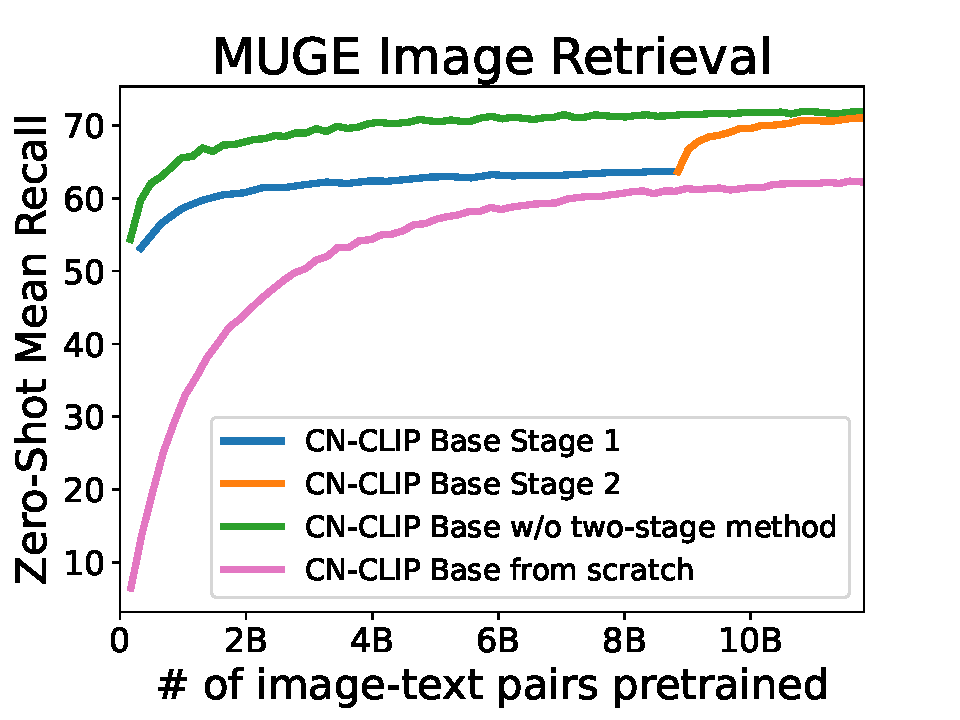
\includegraphics[width=0.97\linewidth]{pics/Mean Recall/MUGE_IR_MR.pdf}
%     }
%     % \caption{Caption}
%     \label{fig:Base MUGE IR}
% \end{figure}
\begin{figure*}
    \centering
    \subfigure[]{
        \begin{minipage}[t]{0.66\columnwidth}
            \label{fig:MUGE IR}
            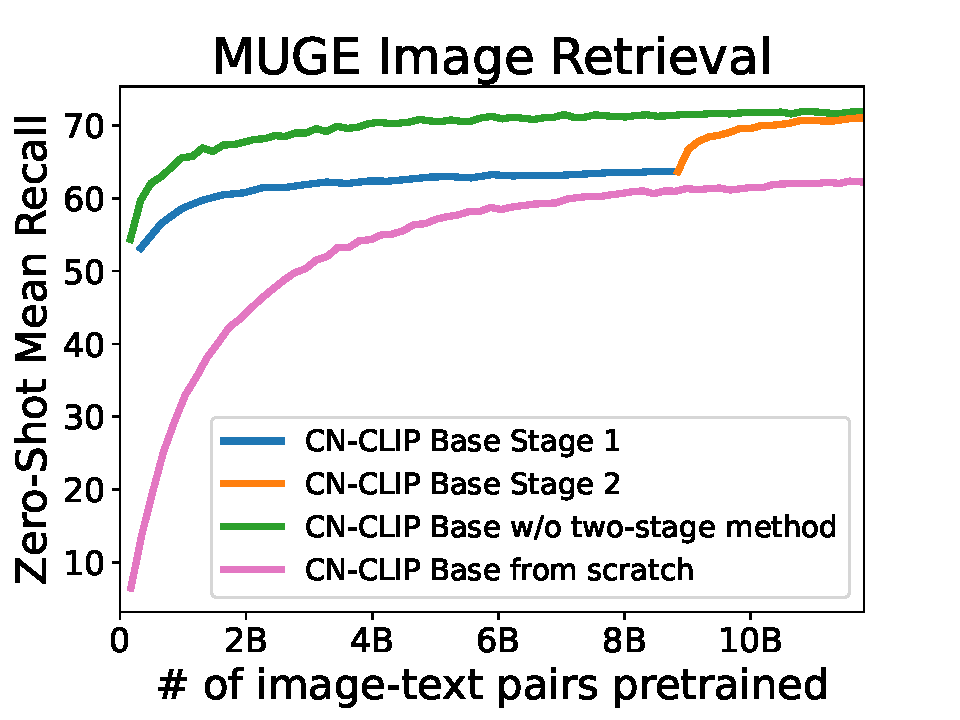
\includegraphics[width=\linewidth]{pics/Mean Recall/MUGE_IR_MR.pdf}
        \end{minipage}
    }
    \subfigure[]{
        \begin{minipage}[t]{0.66\columnwidth}
            \label{fig:Flickr30k-CN IR}
            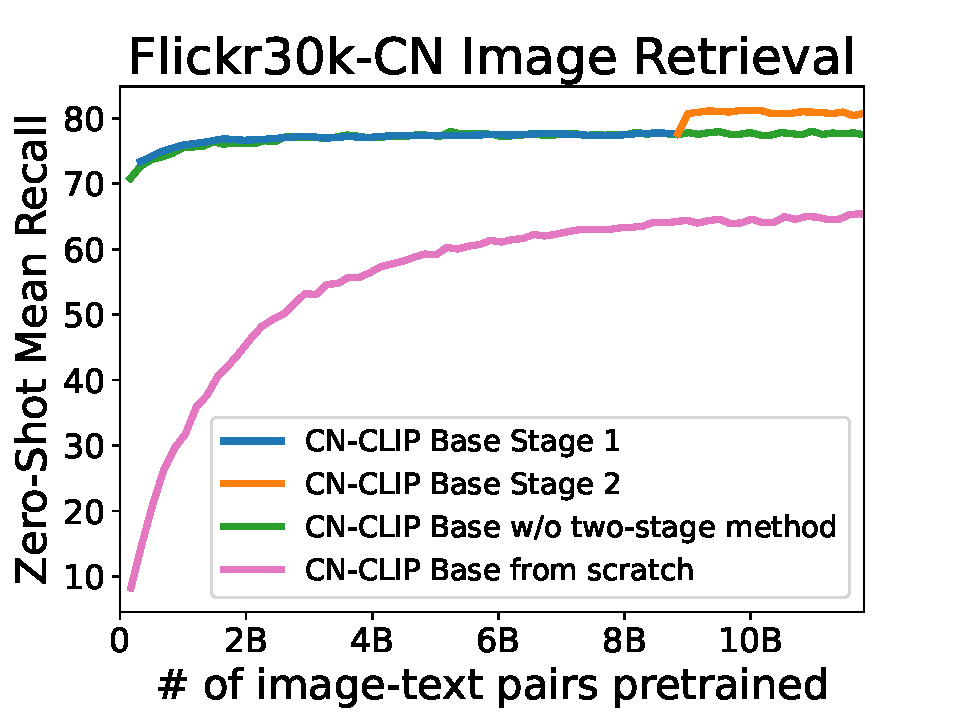
\includegraphics[width=\linewidth]{pics/Mean Recall/Flickr30k-CN_IR_MR.pdf}
        \end{minipage}
    }
    \subfigure[]{
        \begin{minipage}[t]{0.66\columnwidth}
            \label{fig:Flickr30k-CN TR}
            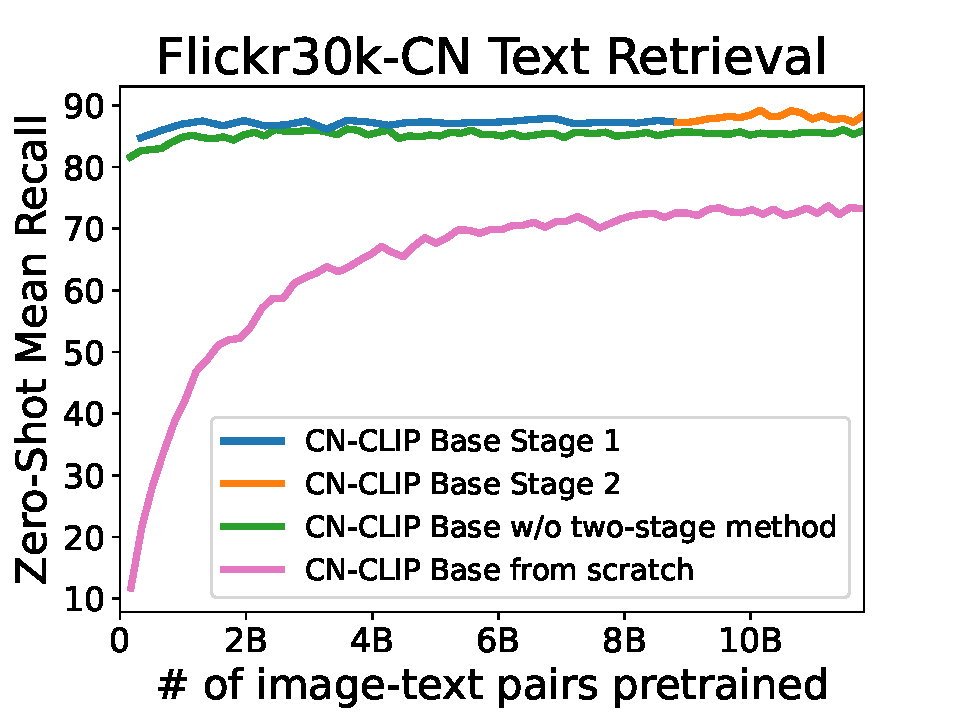
\includegraphics[width=\linewidth]{pics/Mean Recall/Flickr30k-CN_TR_MR.pdf}
        \end{minipage}
    }
    \subfigure[]{
        \begin{minipage}[t]{0.66\columnwidth}
            \label{fig:COCO-CN IR}
            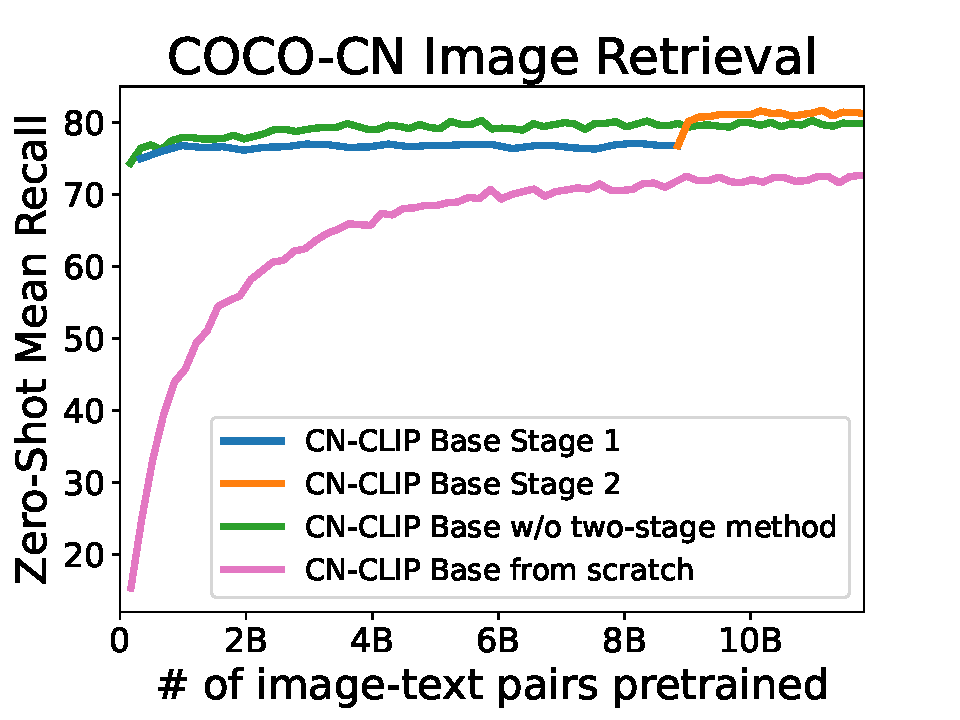
\includegraphics[width=\linewidth]{pics/Mean Recall/COCO-CN_IR_MR.pdf}
        \end{minipage}
    }
    \subfigure[]{
        \begin{minipage}[t]{0.66\columnwidth}
            \label{fig:COCO-CN TR}
            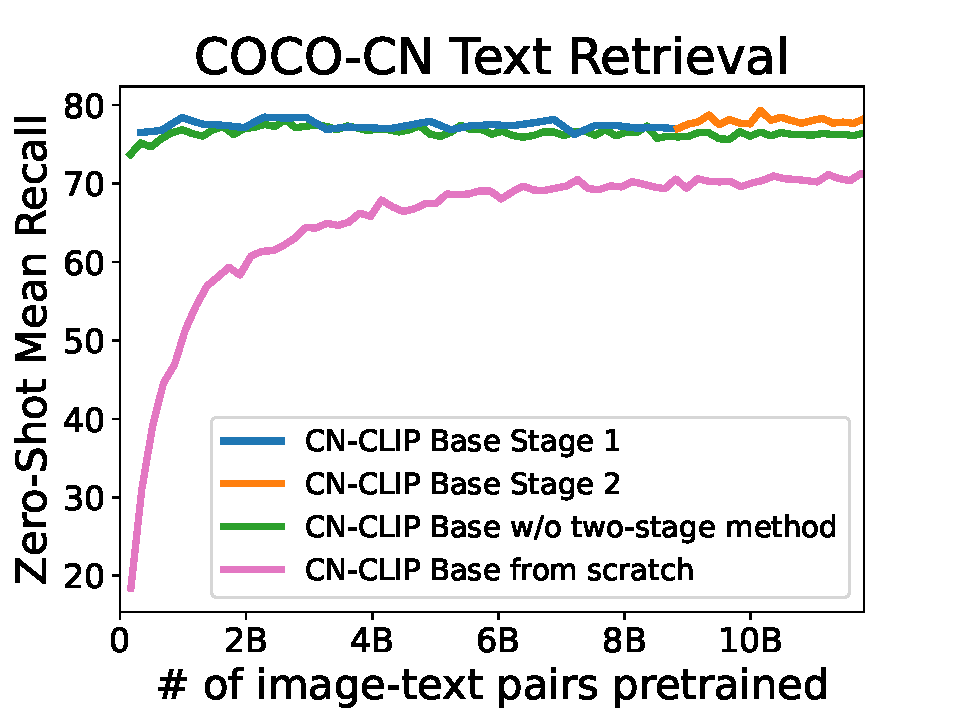
\includegraphics[width=\linewidth]{pics/Mean Recall/COCO-CN_TR_MR.pdf}
        \end{minipage}
    }
    \caption{Comparison of base-size Chinese CLIP models with different training methods on MUGE, Flickr30k-CN and COCO-CN.}
    \label{fig:ablation Base MR}
\end{figure*}

% \begin{figure}
%     \centering
%     \vspace{-0.3cm}
%     \subfigure[]{
%         \begin{minipage}[t]{0.67\linewidth}
%             \label{fig:Flickr30k-CN IR}
%             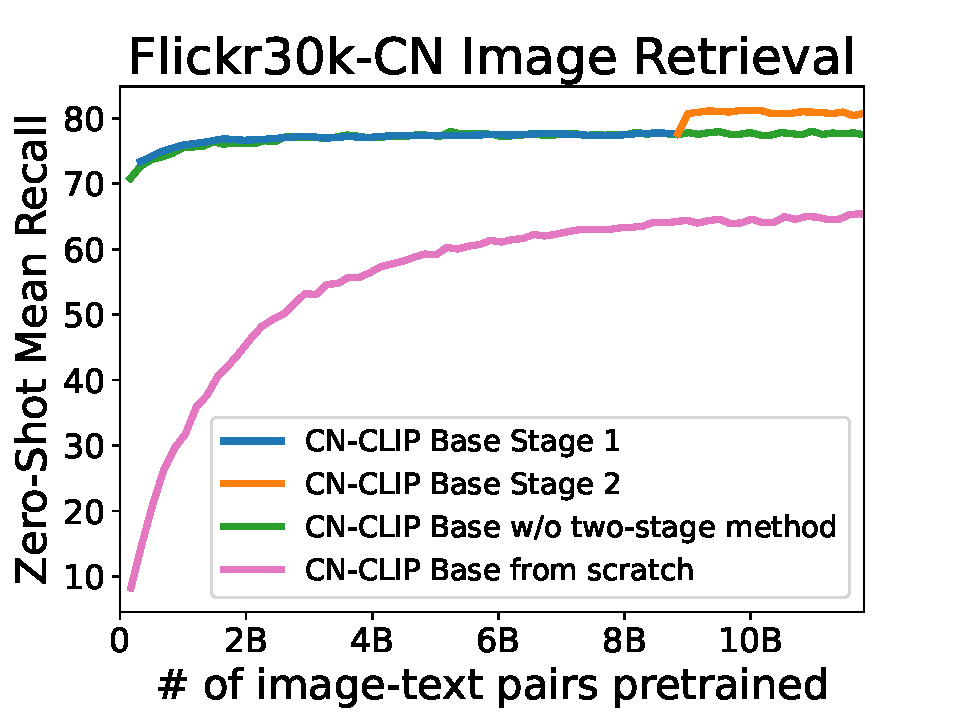
\includegraphics[width=0.97\linewidth]{pics/Mean Recall/Flickr30k-CN_IR_MR.pdf}
%         \end{minipage}
%     }
%     \vspace{-0.3cm}
%     \subfigure[]{
%         \label{fig:Flickr30k-CN TR}
%         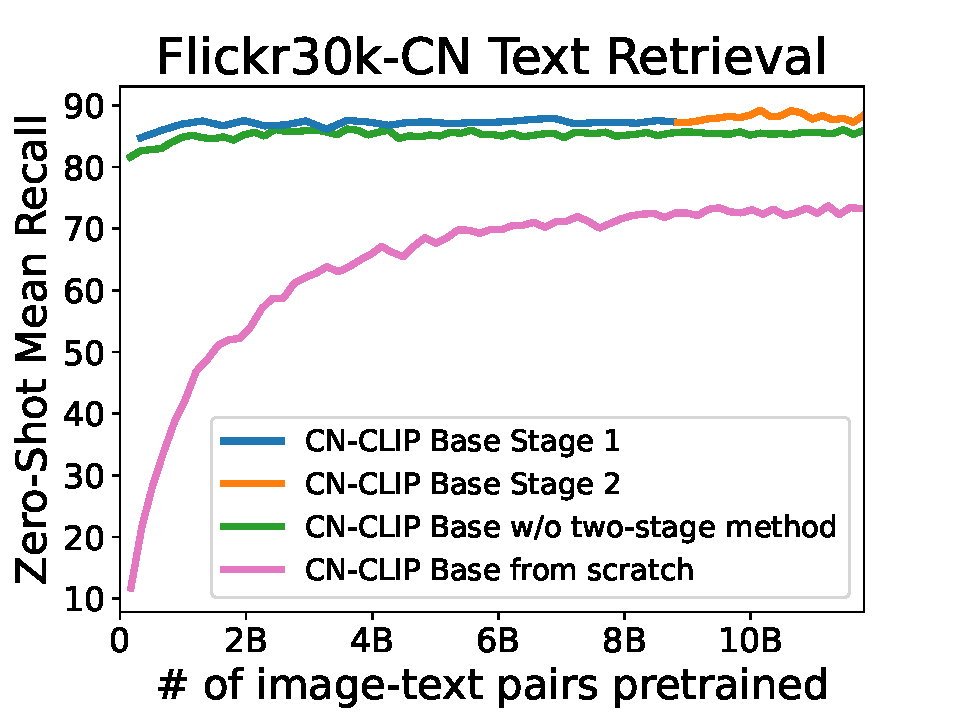
\includegraphics[width=0.97\linewidth]{pics/Mean Recall/Flickr30k-CN_TR_MR.pdf}
%     }
%     \vspace{-0.3cm}
%     \subfigure[]{
%         \label{fig:COCO-CN IR}
%         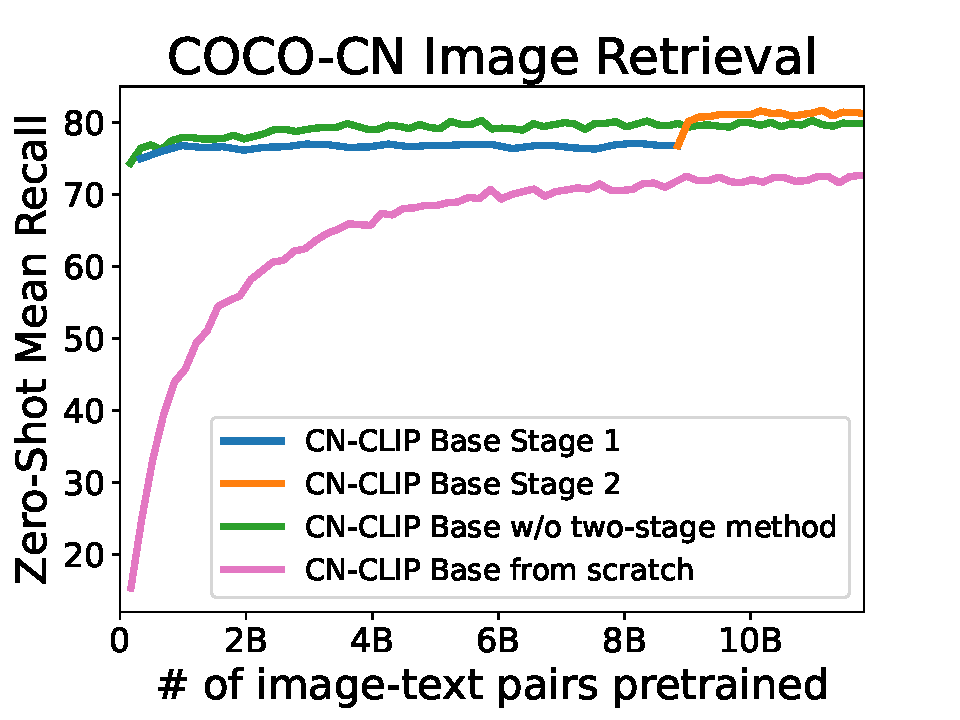
\includegraphics[width=0.97\linewidth]{pics/Mean Recall/COCO-CN_IR_MR.pdf}
%     }
%     \vspace{-0.3cm}
%     \subfigure[]{
%         \label{fig:COCO-CN TR}
%         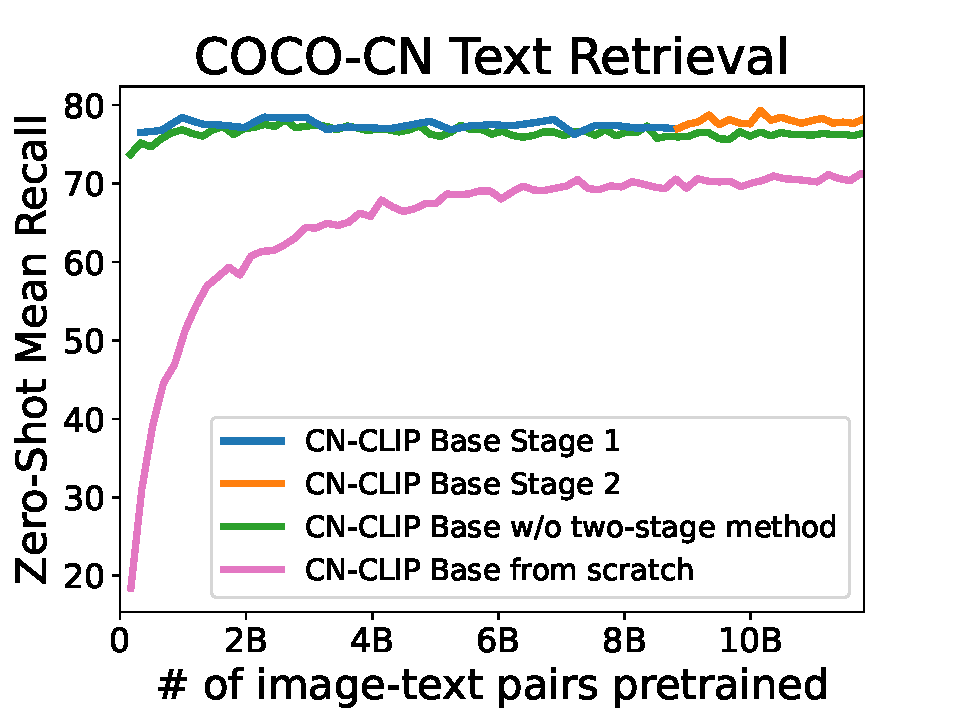
\includegraphics[width=0.97\linewidth]{pics/Mean Recall/COCO-CN_TR_MR.pdf}
%     }
%     \caption{Comparison of the training process of a group of Base scale CLIP models with different training methods on MUGE, Flickr30k-CN and COCO-CN datasets.}
%     \label{fig:Base Flickr30k-CN and COCO-CN MR}
% \end{figure}

\subsubsection{Ablation Study}
Here we provide an ablation study on our proposed two-stage training methods. 
To validate its significance and effectiveness, we design several setups for the ablation study. 
Our experiments are conducted on $\text{CN-CLIP}\rm_{ViT\text{-}B/16}$. 
To evaluate the influence of initialization, we pretrain a model from scratch, and to examine the influence of LiT, we pretrain a model without freezing the image encoder. 
For a better demonstration, we report the curves of model performance of zero-shot retrieval on different datasets in terms of pretraining progress, indicated by the number of processed samples. 

Figure~\ref{fig:ablation Base MR} shows the performance on different tasks, namely MUGE text-to-image retrieval, text-to-image and image-to-text retrieval on Flicrk30K-CN and COCO-CN. 
In comparison with pretraining with pretrained model initialization, pretraining from scratch performs much worse though it shows consistent performance improvement in terms of pretraining progress. 
As to the importance of LiT, we observe different phenomena on different datasets. On MUGE, a dataset of samples originally collected from Chinese websites, we find that pretraining without LiT might be the best solution though its performance gap with two-stage pretraining is quite small. 
However, on the other datasets, i.e., Flickr30K-CN and COCO-CN, whose samples are translated from the English datasets, we find that our two-stage pretraining performs significantly better than pretraining without LiT. 
Furthermore, we observe a common phenomenon that in the two-stage pretraining, switching from Stage 1 to Stage 2 can effectively boost the model performance to a higher level. 
This reflects the importance of adapting the pretrained model to the data distribution of the Chinese multimodal data, especially those concerned with visual information. 

\subsection{Zero-shot Image Classification}
\begin{table*}[t]
\center
\small
\vskip 0.15in
\begin{adjustbox}{max width=1.\textwidth}
\begin{tabular}{@{\extracolsep{\fill}}lccccccccccc}
\toprule
%   Dataset & Metric & $\text{CLIP}\rm_{ViT\text{-}B/32}$ & $\text{CLIP}\rm_{ViT\text{-}B/16}$ & $\text{CLIP}\rm_{ViT\text{-}L/14}$ 
%   & $\text{CN-CLIP}\rm_{RN50}$ & $\text{CN-CLIP}\rm_{ViT\text{-}B/16}$ & $\text{CN-CLIP}\rm_{ViT\text{-}L/14}$ 
%   & $\text{CN-CLIP}\rm_{ViT\text{-}L/14@336px}$ & $\text{CN-CLIP}\rm_{ViT\text{-}H/14}$ 
%   \\
    Model & CIFAR10 & CIFAR100 & DTD & EuroSAT & FER & FGVC & KITTI & MNIST & PC & VOC & INet\\
\midrule
    \multicolumn{8}{l}{\textit{Original benchmark}} \\
    DeCLIP  & 90.9 & 66.8 & 44.9 & 39.9 & 23.3 & 9.0 & 39.7 & 13.6 & 55.3  & 80.6 & 73.7\\
    GIT  & 88.5 & 61.1 & 42.9 & 43.4 & 41.4 & 6.7 & 22.1 & 68.9 & 50.0 & 80.2 & -\\
    % $\text{ALIGN}\rm_{ViT\text{-}B}$ & 88.1 & 60.3 & 44.9 & 14.8 & 46.6 & 62.1 & 53.1 & 82.8\\
    ALIGN & \textbf{94.9} & 76.8 & \textbf{66.1} & 52.1 & \textbf{50.8} & 25.0 & \textbf{41.2} & 74.0 & 55.2 & 83.0 & \textbf{76.4}\\
    % $\text{CLIP}\rm_{ViT\text{-}B/32}$ & Scale & CIFAR-10 & CIFAR-100 & FER & FGVC & KITTI & MNIST & PatchCamelyon & Cars & VOC\\
    OpenCLIP  & 93.5 & 76.2 & 56.4 & 53.7 & 50.3 & 20.8 & 28.8 & 70.9 & 50.5 & 82.3 \\
    CLIP  & \textbf{94.9} & \textbf{77.0} & 56.0 & \textbf{63.0} & 48.3 & \textbf{33.3} & 11.5 &\textbf{79.0} & \textbf{62.3} & \textbf{84.0} & 76.2\\
\midrule
    \multicolumn{8}{l}{\textit{Translated benchmark}} \\
    BriVL  & 72.3 & 35.9 & 18.8 & 25.5 & - & - & - & - & -  & - & 24.3\\
    Wukong & 95.4 & 77.1 & 40.9 & 50.3 & - & - & - & - & -  & - & 55.0\\
    CN-CLIP & \textbf{96.0} & \textbf{79.7} & \textbf{51.2} & \textbf{52.0} & \textbf{55.1} & \textbf{26.2} & \textbf{49.9} & \textbf{79.4} & \textbf{63.5} & \textbf{84.9} & \textbf{59.6} \\
\bottomrule
\end{tabular}
\end{adjustbox}
\caption{Experimental results of the zero-shot image classification performance of models on ICinW. }
\label{tb:zs_v2}
\end{table*}

% Caltech-101 & 87.5 & 88.9 & \textbf{92.4} & 77.3 & 84.9 & 88.5 & 88.8 & 90.6  \\
%   CIFAR-10  & 89.9 & 90.8 & 94.9 & 72.7 & 92.0 & 94.9 & 94.1 & \textbf{96.0}  \\
%   CIFAR-100  & 65.1 & 68.2 & 77.0 & 40.6 & 64.4 & 75.1 & 73.5 & \textbf{79.7}  \\
%   Country-211  & 17.2 & 22.8 & \textbf{34.5} & 7.7 & 15.2 & 21.0 & 25.4 & 25.3  \\
%   DTD  & 44.4 & 44.7 & \textbf{56.0} & 36.9 & 43.6 & 44.2 & 43.8 & 51.2  \\
%   EuroSAT  & 45.6 & 54.7 & \textbf{63.0} & 27.0 & 46.9 & 56.9 & 50.7 & 52.0  \\
%   FER-2013  & 42.1 & 48.5 & 48.3 & 21.9 & 47.2 & 54.6 &\textbf{ 55.1} & 49.2  \\
%   FGVC-Aircraft  & 19.6 & 24.3 & \textbf{33.3} & 5.4 & 12.8 & 16.0 & 17.1 & 26.2  \\
%   Food-101  & 84.0 & 88.7 & \textbf{93.9} & 39.8 & 62.4 & 69.4 & 73.9 & 74.6  \\
%   GTSRB  & 32.8 & 43.6 & \textbf{52.3} & 22.3 & 28.4 & 37.3 & 35.5 & 38.5  \\
%   Hateful-Memes  & 56.0 & 58.1 & \textbf{60.0} & 50.3 & 56.2 & 53.4 & 52.8 & 54.7  \\
%   KITTI-Distance  & 29.0 & 26.7 & 11.5 & 30.2 & 33.5 & 49.9 & \textbf{49.8} & 39.1  \\
%   MNIST  & 48.1 & 52.1 & 79.0 & 50.2 & 67.6 &69.8 & 65.0 & \textbf{79.4}  \\
%   Oxford Flowers-102  & 66.5 & 69.4 & \textbf{78.5} & 30.7 & 52.2 &62.5 & 64.8 & 68.4  \\
%   Oxford-IIIT Pets  & 87.1 & 89.0 & \textbf{93.8} & 48.7 & 73.0 &81.6 & 83.1 & 83.5  \\
%   PatchCamelyon  & 60.7 & 54.0 & 62.3 & 47.7 & 54.0 &\textbf{63.5} & 62.9 & 52.4  \\
%   Rendered-SST2  & 58.4 & 60.6 & \textbf{70.6} & 50.1 & 52.3 & 61.4 & 62.9 & 61.0  \\
%   RESISC-45  & 60.0 & 65.6 & \textbf{71.4} & 49.3 & 58.7 & 65.2 & 65.8 & 66.9  \\
%   Stanford-Cars  & 59.7 & 64.8 & \textbf{79.3} & 27.3 & 42.3 &49.8 & 54.1 & 71.8  \\
%   VOC-2007  & 82.6 & 83.7 & 84.0 & 82.1 & 83.3 & 84.5 & \textbf{84.9} & \textbf{84.9}  \\
%   Average & 56.8 & 60.0 & \textbf{66.8} & 40.9 & 53.5 & 60.0 & 60.2 & 62.3  \\
% This section introduces the image classification datasets, and provides comprehensive experimental results and in-depth analyses to probe the inherent defects of Chinese CLIP. 

\subsubsection{Open-Domain Image Classification Benchmark in Chinese}
Contrastive pretraining on image-text pairs builds a connection between vision and natural language. Natural language supervision instead of crowd-sourced labeling endows models with the capability of zero-shot image classification by computing similarities between the given image and the text descriptions of the labels in the candidate set. 
Recent progress in this field is the ELEVATER benchmark~\citep{elevater}. 
The track ICinW for open-domain image classification consists of a series of image classification datasets, including ImageNet~\citep{imagenet}, CIFAR~\citep{cifar}, MNIST~\citep{mnist}, etc.
%  e.g., CIFAR-10, CIFAR-100~\citep{cifar}, DTD~\citep{dtd}, EuroSAT~\citep{eurosat}, FER-2013~\citep{clip}, FGVC-Aircraft~\citep{fgvc}, KITTI-Distance~\citep{kitti}, MNIST~\citep{mnist}, Pascal-VOC-2007~\citep{voc}, etc. 
% The evaluation metrics include accuracy, mean-per-class, etc. 
% More details about the datasets and metrics are reported in the appendix. 
In order to evaluate Chinese CLIP on the datasets, we first transform the datasets for Chinese models by translating labels and prompts into Chinese. 
% Specifically, we translate the text descriptions of the labels and the templates for manual prompts to Chinese. 
% For example, the labels in CIFAR-10 include ``car, dog, ...'', and we manually translate the words into Chinese. 
% There are also particular cases, such as the labels in FGVC-Aircraft~\citep{fgvc}, which it is difficult to translate or transliterate. 
% We search the names on Google and figure out the best Chinese name for each label. 
% Be that as it may, we cannot guarantee that we have the best Chinese translation, and more importantly, it is still hard for the Chinese pretrained model to understand some of the concepts, which may lead to unsatisfactory performance in the related downstream tasks. 
% As to the templates, for some datasets, we use our translation of the templates provided by the ELEVATER toolkit,\footnote{https://github.com/Computer-Vision-in-the-Wild/Elevater\_Toolkit\_IC} and for the others, we use the translation of the templates from OpenAI CLIP.~\footnote{The organized datasets with translated labels and templates will be released. }

\subsubsection{Experimental Results}
Table~\ref{tb:zs_v2} reports the performance of both English models and Chinese models. 
The baselines pretrained on English data include DeCLIP~\citep{declip}, ALIGN~\citep{align}, CLIP~\citep{clip}, and OpenCLIP~\citep{openclip}, and the baselines pretrained on Chinese data include BriVL~\citep{wenlan} and Wukong~\citep{wukong}. 
We report the results of the variant with the best downstream performance for the models. 

We first focus on the comparison with the Chinese baselines. 
% Chinese CLIP outperforms both baselines on the $4$ datasets significantly. 
% To be specific, Chinese CLIP surpasses BriVL and Wukong by $23.7$ and $0.6$ on CIFAR-10, $43.8$ and $2.6$ on CIFAR-100, $32.4$ and $10.3$ on DTD, and $26.5$ and $1.7$ on EuroSAT. 
To be specific, on all datasets including ImageNet classification, Chinese CLIP surpasses both baselines significantly, and the relative achievements on some datasets are over $100\%$. 
Besides, we also compare Chinese CLIP with the foundation models, e.g., CLIP and ALIGN, which are pretrained on English data. 
It can be found that Chinese CLIP outperforms CLIP or ALIGN on CIFAR-10, CIFAR-100, FER-2013, KITTI-Distance, MNIST, PatchCamelyon, and Pascal-VOC-2007. 
Also, on the classification datasets for general concepts or objects common in both western and eastern culture, Chinese CLIP consistently achieves better performance. 
This indicates that Chinese CLIP is capable of categorizing images to general prototypes. 

However, as to the classification concerned with proper nouns, e.g., FGVC-Aircraft, it is difficult for all models to achieve high accuracy. 
We assume that the related images and texts are not common in the pretraining datasets, and it is also hard for the models to understand the names of airplanes without finetuning. 
Specifically, for Chinese models, the translation or even transliteration can significantly affect the performance of Chinese CLIP. It encourages building a benchmark of ``Image Classification in the Wild for Chinese Models''. 

% Experimental results show that on the $4$ datasets, namely CIFAR-10, CIFAR-100, DTD, and EuroSAT, Chinese CLIP
% The results of the baseline models are provided by the official website of ICinW, which is a direct evaluation of OpenAI CLIP. 
% To be more specific, we report the scores of $\text{CLIP}\rm_{ViT\text{-}B/32}$, $\text{CLIP}\rm_{ViT\text{-}B/16}$, and $\text{CLIP}\rm_{ViT\text{-}L/14@336px}$. 
% As to the average performance on the datasets, the large-size and huge-size Chinese CLIP models, including $\text{CN-CLIP}\rm_{ViT\text{-}L/14}$, $\text{CN-CLIP}\rm_{ViT\text{-}L/14@336px}$, and $\text{CN-CLIP}\rm_{ViT\text{-}H/14}$, can outperform the base-size baselines $\text{CLIP}\rm_{ViT\text{-}B/32}$ and $\text{CLIP}\rm_{ViT\text{-}B/16}$. 
% In comparison with the large-size baseline $\text{CLIP}\rm_{ViT\text{-}L/14@336px}$ pretrained on data of larger resolution $336 \times 336$, the huge-size $\text{CN-CLIP}\rm_{ViT\text{-}H/14}$ outperforms it in several datasets, e.g., CIFAR-10, CIFAR-100, MNIST, and VOC-2007, which are related to the image classification of common objects and general prototypes. 
% This reflects the potential of Chinese CLIP on the understanding of general concepts. 
% Besides, the quality of translation makes a difference in this scenario. 
% There are a number of labels that may not have proper translations in Chinese, or to say, translations that the Chinese language models can understand. 
% For example, most names of airplanes and cars can only be translated into Chinese by transliteration. 
% The language models cannot understand the concepts if their frequencies are low in the corpora. 
% Another problem is that the images of many categories of this benchmark are rare in the Chinese data. 
% To be more specific, many images in some datasets, e.g., Country-211 for country classification, Flowers-102 and Oxford-Pets for the classification of flowers and pets, are quite rare in our pretraining data mostly crawled from the Chinese websites. 
% This finding is consistent with our motivation about why it is necessary to build a language-specific cross-modal pretrained model. 
% Also, it encourages building a benchmark of ``Image Classification in the Wild for Chinese Models''. 


\subsubsection{Analysis}
% Here we illustrate some findings of Chinese CLIP in the experiments, including the sensitivity to handcrafted prompts and the inability to understand negation. 

\paragraph{Sensitivity to Handcrafted Prompts}
While the benchmark ELEVATER provides specific prompts for each dataset, we find that this is not always the best option, in comparison with our baseline, translation of the prompts provided by OpenAI CLIP. 
% Although the accumulation of manual prompts does not consistently improve performance, 
The baseline with around $90$ prompts performs the best on average. 
However, for some datasets, specific prompts designed with human knowledge can boost the performance significantly. 
A typical case is the classification of airplanes. 
We test $\text{CN-CLIP}\rm_{ViT\text{-}L/14}$ with our specified prompts that are related to the knowledge of aircraft, e.g.,``{label}, a photo of an airplane", ``{label}, a zoomed image of a fighter'', etc., and the translation of the OpenAI prompts.
Experimental results show that the model can achieve an accuracy of $16.0$ with the specified prompts but only $13.8$ with the OpenAI prompts. 
% Similar phenomena also happen in other datasets. 
% We list more results in the appendix. 


\paragraph{Inability to Understand Negation}
Previous studies~\citep{negbert, bertnot} demonstrate that even strong NLP pretrained models  often make mistakes in negation problems. 
We explore CLIP's capability to understand negation by conducting experiments on KITTI-Distance~\citep{kitti} and PatchCamelyon~\citep{patchcamelyon}. 
KITTI-Distance provides $4$ options for models to judge, including ``next to a car'', ``near a car'', ``at a distance away from a car'', and ``no car''. The last one is concerned with negation. 
We compare the model performance using the text ``no cars'' and ``others'' for the last label. 
We observe that it is hard for the model to understand negation. By changing the label from ``others'' to ``no cars'', the performance drops by $48.1\%$ in accuracy ($49.9$ vs. $25.9$). 
Similarly, in the experiments on PatchCamelyon, the performance drops from $63.5$ to $50.2$ by changing labels from ``mainly red'' and ``green block in the middle'' to ``no green block in the middle'' and ``green block in the middle''. 
This shows the limitation of the training of CLIP in learning negation. 
The texts in the pretraining datasets are mostly descriptions of the images, which indicate their objects or features but often do not indicate the absence of objects. 
% In the future research, we will explore heuristically building datasets with negation. For example, we sample objects that are not present in an image, construct a text description for negation with manual templates, and train CLIP models on such datasets. 


\subsection{Deployment}
For deployment, we develop ONNX-based and TensorRT-based models based on our Pytorch-based pretrained Chinese CLIP models. 
As expected, we observe that the inference efficiency increases significantly while there is almost no performance sacrifice. 
Specifically, the inference efficiency of TensorRT-based models is around $2$ to $10$ times faster than the Pytorch-based models. More statistics are listed in Appendix~\ref{appendix:deployment}. 